\documentclass[a4paper,10pt]{article}
\usepackage[utf8]{inputenc}
\usepackage[brazilian]{babel}
\usepackage[margin=0cm]{geometry}
\usepackage{graphicx}
\usepackage{xcolor}
\usepackage{tikz}
\usepackage{multicol}
\usepackage{caption}
\usepackage{enumitem}
\usepackage[numbers]{natbib}
\usepackage{amsmath}
\usepackage{helvet}
\renewcommand{\familydefault}{\sfdefault}
\setlength{\parindent}{0pt}
\setlength{\parskip}{3pt}
\begin{document}
\begin{tikzpicture}[remember picture, overlay]

    \node[anchor=north west, inner sep=0pt] at (current page.north west) {
        
\includegraphics[width=\paperwidth, height=4.0cm]{images/banner-2022-prt-superior-2_amostra-cientifica_tecnologica-e-cultural.png}
    };
    \node[anchor=south west, inner sep=0pt] at (current page.south west) {
        
\includegraphics[width=\paperwidth, height=4.8cm]{images/banner-2022-prt-infeior_realizado-eapoiador_2022.png}
    };

\end{tikzpicture}
\vspace*{3.2cm}

\begin{center}
    {\bfseries\scriptsize GOVERNO DO ESTADO DO RIO GRANDE DO NORTE}\\[0.3mm]
    {\bfseries\scriptsize SECRETARIA ESTADUAL DA EDUCAÇÃO, DA CULTURA, DO ESPORTE E DO LAZER - SEEC}\\[0.3mm]
    {\bfseries\scriptsize 6ª DIREC - DIRETORIA REGIONAL DA EDUCAÇÃO, DA CULTURA E DOS ESPORTES}\\[0.3mm]
    {\bfseries\scriptsize CENTRO ESTADUAL DE EDUCAÇÃO PROFISSIONAL PROF.ª MARIA RODRIGUES GONÇALVES - CEEP-PMRG}\\[2.5mm]
    {\bfseries\large ANÁLISE E PROPOSTA DE ADEQUAÇÃO DO LABORATÓRIO DE INFORMÁTICA DO CEEP-PMRG}\\[1.5mm]
    {\bfseries\scriptsize ARAÚJO, A. F. G. de.; ALVES, D. S. G.; PIMENTEL, F. P.; ARAÚJO, F. L. de.; CARDOSO, J. V.}
\end{center}
\vspace{0.2cm}
\noindent\centering
\begin{minipage}{0.92\paperwidth}
\begin{multicols}{2}
\scriptsize
\tolerance=9999
\emergencystretch=3em
\hyphenpenalty=50
\exhyphenpenalty=50
\section*{\centering INTRODUÇÃO}

A utilização de laboratórios de informática nas escolas estaduais do Rio Grande do Norte tem sido de suma importância para o ensino e a aprendizagem de estudantes das escolas técnicas, pois contribui significativamente para a aprendizagem e para a formação acadêmica, já que adquirem conhecimentos por meio das tecnologias implementadas nas instituições de ensino. O Ministério da Educação (MEC), em parceria com os governos estaduais e municipais, promoveu a implementação e o uso dessas tecnologias por meio dos laboratórios de informática, através do Programa Nacional de Tecnologia Educacional (ProInfo)~\cite{proinfo1997} em instituições de ensino~\cite{lobler2012renote}.
Com isso em mente, este trabalho aponta a importância da adequação do Laboratório de Informática do CEEP-PMRG, como fonte de melhoria no processo de aprendizagem dos estudantes da base técnica de ensino da instituição. Desse modo, o estudo teve como objetivo geral produzir uma planta baixa para adequação do Laboratório de Informática.
\section*{\centering REFERENCIAL TEÓRICO}

Por ser um recurso de grande relevância para a aprendizagem, os laboratórios de informática estão cada vez mais presentes no âmbito educacional, tendo em vista que a informatização faz parte do dia a dia da sociedade. A construção deste referencial teórico baseia-se na documentação da Cartilha do ProInfo~\citep{proinfo1997}, realizando-se um comparativo entre as normas do que é adequado para um laboratório de informática e o que as instalações e padronizações do CEEP-PMRG oferecem.
A norma abrange a estrutura e o espaço do laboratório de informática, os computadores, o mobiliário e as instalações elétricas e de rede. O espaço é fundamental para o ambiente, pois deve ser adequado para a distribuição do mobiliário e demais especificações, visando evitar dificuldades durante a locomoção no local ou o manuseio dos equipamentos, como mouse e teclado. A distribuição das instalações elétricas e de rede deve corresponder à quantidade de computadores, garantindo que todos possam ser utilizados e tenham acesso à internet. Dessa forma, contribui-se para o ensino e para a aprendizagem.
\section*{\centering METODOLOGIA}

A abordagem de pesquisa para a construção do presente trabalho é qualitativa, pois busca compreender a importância da correta adequação do laboratório de informática como recurso mediador da aprendizagem nos cursos Técnicos em Informática. Quanto aos objetivos, o estudo classifica-se como uma pesquisa descritiva — visto que busca abordar uma série de informações coletadas por meio do método de pesquisa bibliográfica, selecionando artigos e monografias que trazem ideias construtivas para embasar o tema exposto, de forma seletiva e analítica — e explicativa, pois defende a hipótese de que a adequação na estrutura desse ambiente pode influenciar o ensino e a aprendizagem de maneira positiva, caso esteja de acordo com o que é recomendado pelas normas técnicas para os laboratórios.
Quanto aos procedimentos, o método empregado caracteriza-se como uma pesquisa experimental, que busca compreender a realidade enfrentada na estrutura do Laboratório de Informática do CEEP-PMRG, propondo a produção de uma planta baixa diante da realidade encontrada, com o intuito de propor melhorias para o ensino nesse ambiente.
\section*{\centering RESULTADOS E DISCUSSÕES}

O presente trabalho resultou na elaboração de uma planta baixa com as devidas adequações para o Laboratório de Informática do CEEP-PMRG, destacando as instalações elétricas e de rede, bem como a distribuição do mobiliário, dos computadores, da climatização e dos materiais necessários para o seu funcionamento.
Para a composição ideal desse ambiente, propos-se uma área total de 25 m × 7 m, dividida em Sala 1 (20 m de comprimento) e Sala 2 (5 m de comprimento), garantindo espaço adequado para comportar o mobiliário e os equipamentos. Quanto ao mobiliário, este deve ser distribuído em duas fileiras de 4 mesas, a fim de assegurar o espaçamento de 30 cm entre cada computador. Com relação às instalações elétricas e de rede, elas devem atender à quantidade de computadores existentes no laboratório. Além disso, o ambiente precisa estar bem estruturado para que todos os computadores funcionem com acesso à internet e distribuição adequada de energia.
\vspace{0.1cm}
\begin{center}
    \begin{minipage}{\linewidth}
        \centering
        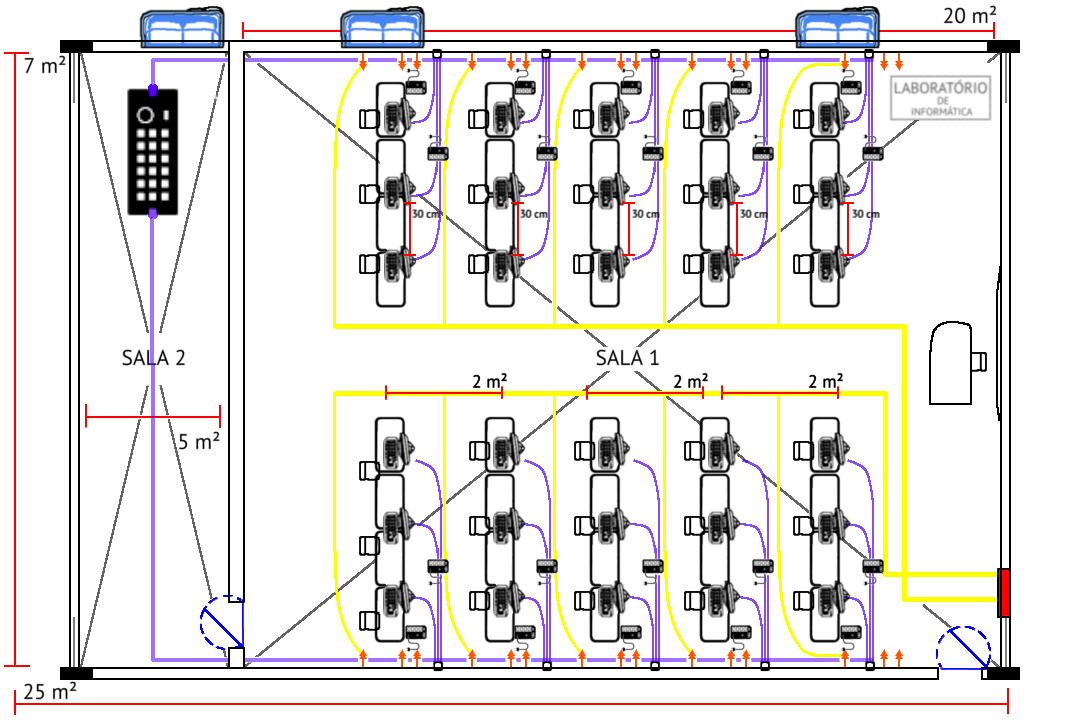
\includegraphics[width=\linewidth, keepaspectratio]{figures/figura-01_planta-lab-adequada-prop.png}
        \label{fig:planta_baixa}
    \end{minipage}
\end{center}
\vspace{0.1cm}
\section*{\centering CONSIDERAÇÕES FINAIS}

Com o planejamento e a construção da planta baixa do Laboratório de Informática do Centro Estadual de Educação Profissional Professora Maria Rodrigues Gonçalves, foi possível concluir que a implementação das normas torna o ambiente mais produtivo e padronizado. Ao transformar a realidade encontrada, aumenta-se o interesse dos estudantes da base técnica em Informática — e também de outros cursos — em estudar e realizar as práticas necessárias que o espaço oferece. Além disso, os professores da base técnica sentem-se motivados para a aplicação de novas metodologias de ensino como mecanismo de aprendizagem.
\section*{\centering REFERÊNCIAS}
\renewcommand{\refname}{}
\bibliographystyle{plainnat}
\bibliography{references}
\end{multicols}
\end{minipage}
\end{document}